\documentclass{article}
\usepackage{graphicx} % Required for inserting images
\usepackage{amsmath}
\title{CSC376 - ASSIGNMENT 1}
\author{Jott Girn and Stephen Le}
\date{October 2024}

\begin{document}
 \maketitle 
Each question is listed below.\\
\textbf{Question 1}:\\
\begin{enumerate}
    \item \begin{itemize}
        \item First, let us consider the displacement from $w$ to $c$, which, looking at the visual, is $F$ in the x direction, $D$ in the y direction, and $E$ in the z direction. Looking at the axis, it can be seen that the $x$ and $y$ axis are both opposite by $\pi$ radians on the $z$ axis, using the common rotation matrices, we can solve:
        \begin{align}
            T_{wc} &= \begin{bmatrix}
R & p \\
0 & b 
\end{bmatrix}\\
&= \begin{bmatrix}
cos(\pi) & -sin(\pi)& 0 & F \\
sin(\pi) & cos(\pi) & 0 & D \\
0 & 0 & 1& E \\
0 & 0 & 0 & 1
\end{bmatrix}\\
&= \begin{bmatrix}
-1 & 0& 0 & F \\
0 & -1 & 0 & D \\
0 & 0 & 1& E \\
0 & 0 & 0 & 1
\end{bmatrix}
        \end{align}
    \end{itemize}
    \item Note that both $p_1$ and $p_2$ have no rotation on the axis, and are simply displaced on the $y$ axis by a total of $4L+A$ units, using this, let us compute:
    the $z$ axis, using the common rotation matrices, we can solve:
        \begin{align}
            T_{p_1p_2} &= \begin{bmatrix}
0 & 0& 0 & 0 \\
0 & 0 & 0 & -(A+4L) \\
0 & 0 & 0& 0 \\
0 & 0 & 0 & 1
\end{bmatrix}
        \end{align}
        \item Let us simply apply the properties of matrices:
        \begin{align}
            T_{bc} &= T_{bs}T_{sc}\\
            &= (T_{sb})^{-1}T_{sw}T_{wc}\\
            &= (T_{sb})^{-1}(T_{ws})^{-1}T_{wc}
        \end{align}

From the question, the matrice $T_{ws}$ is known, alongside $T_{sb}$, while $T_{wc}$ is known from part a.
\item First, notice the displacement, which is $5L$ in the x direction, nothing in the y direction, and $H$ in the z direction. Also, notice that the axis is rotated by $\pi/2$ around the z axis, putting this together:
\begin{align}
            T_{p_1box_1} &= \begin{bmatrix}
R & p \\
0 & b 
\end{bmatrix}\\
&= \begin{bmatrix}
cos(\pi/2) & -sin(\pi/2)& 0 & 5L \\
sin(\pi/2) & cos(\pi/2) & 0 & 0 \\
0 & 0 & 1& H \\
0 & 0 & 0 & 1
\end{bmatrix}\\
&= \begin{bmatrix}
0 & -1& 0 & 5L \\
1 & 0 & 0 & 0 \\
0 & 0 & 1& H \\
0 & 0 & 0 & 1
\end{bmatrix}
        \end{align}
\item Note how from $p_1$, box 16 is $5L$ on the x axis, $3L$ on the $Y$ axis, and $H$ on the Z axis, while keeping the same rotations as before:
\begin{align}
            T_{p_1box_{16}} &= \begin{bmatrix}
R & p \\
0 & b 
\end{bmatrix}\\
&= \begin{bmatrix}
cos(\pi/2) & -sin(\pi/2)& 0 & 5L \\
sin(\pi/2) & cos(\pi/2) & 0 & 3L \\
0 & 0 & 1& H \\
0 & 0 & 0 & 1
\end{bmatrix}\\
&= \begin{bmatrix}
0 & -1& 0 & 5L \\
1 & 0 & 0 & 3L \\
0 & 0 & 1& H \\
0 & 0 & 0 & 1
\end{bmatrix}
        \end{align}
\item
Consider the path from $c$ to $p_{50}$, let us break it down in terms of more known matrices:
\begin{align}
    T_{cp_{50}} &= T_{cw}T_{wp_{50}}\\
    &= (T_{wc})^{-1}T_{wp_1}T_{p_1p_{50}}
\end{align}
Now, from the previous questions and information, $T_{wc}$ and $T_{wp_1}$ are known, so all that needs to be solved is $T_{p_1p_50}$, consider the following drawing:
\begin{center}
            \includegraphics[scale=0.75]{boxes.png}
        \end{center}
The reference for the $50th$ box is $H+3L$ in the z direction, $L$ in the x direction, and nothing in the y direction, while still applying the same rotation in the previous box questions:
\begin{align}
            T_{p_1p_50} &= \begin{bmatrix}
R & p \\
0 & b 
\end{bmatrix}\\
&= \begin{bmatrix}
cos(\pi/2) & -sin(\pi/2)& 0 &  L \\
sin(\pi/2) & cos(\pi/2) & 0 & 0 \\
0 & 0 & 1& H+3L \\
0 & 0 & 0 & 1
\end{bmatrix}\\
&= \begin{bmatrix}
0 & -1& 0 & L \\
1 & 0 & 0 & 0 \\
0 & 0 & 1& H+3L \\
0 & 0 & 0 & 1
\end{bmatrix}
        \end{align}
Now, all three matrices are known, and the matrix can be solved for such that:
\begin{align}
    T_{cp_50} &= (T_{wc})^{-1}T_{wp_1}T_{p_1p_{50}} \\
    &= (T_{wc})^{-1}T_{wp_1}\begin{bmatrix}
0 & -1& 0 & L \\
1 & 0 & 0 & 0 \\
0 & 0 & 1& H+3L \\
0 & 0 & 0 & 1
\end{bmatrix}
\end{align}
Now, $T_{ws}$ is given in the question, $T_{wp_1}$ as well, while $T_{p_1box_1}$ was determined in above.
\item Let us simplify this matrix further:
\begin{align}
    T_{sbox_1} &= T_{sp_1}T_{p_1box_1} \\
    &= T_{sw}T_{wp_1}T_{p_1box_1}\\
    &= (T_{ws})^{-1}T_{wp_1}T_{p_1box_1}
\end{align}
These are all known from previous questions or given to be known in the question.
        \end{enumerate}
\textbf{Question 2}:\\

\begin{align}
    \begin{array}{c|lcrr}& \alpha_{i-1} & a_{i-1} &  d_{i}  & \phi _{i}
\\\hline1 & 0 & 0 & \theta_1 +L_0 & 0
\\2 & \pi/2 & L_2 & 0 & \pi/2 + \theta_2
\\3 & \pi/2  & 0 & L_2 & \pi/2
\\4 & 0  & 0 & L_3+\theta_3 & \theta_4
\end{array} 
\end{align}
\textbf{Question 3}:\\
Note that I used "DH parameters", either was accepted and we had this checked over with the professor and TA office hours, here's our diagram below, alongside the code:
\begin{center}
            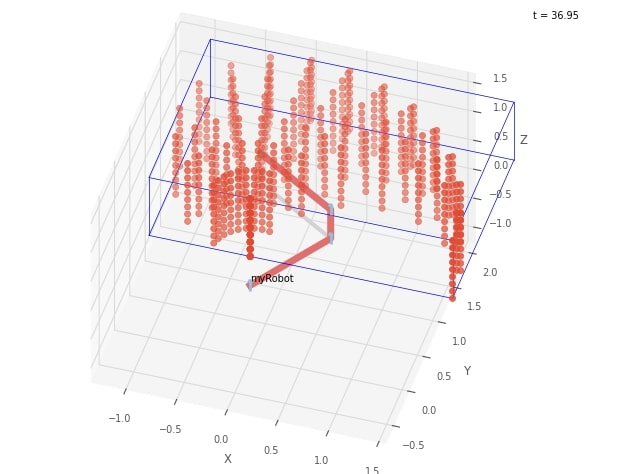
\includegraphics[scale=0.5]{workspace.jpg}
        \end{center}
\end{document}
